\begin{figure}
	\centering
	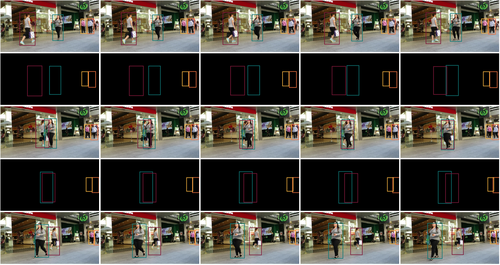
\includegraphics[width=1.0\textwidth]{figures/MOHART/mot_example1.png}
	\caption{Camera blackout experiment on a pedestrian street scene from the MOTChallenge dataset without ego-motion. Subsequent frames are displayed going from top left to bottom right. Shown are the inputs to the model (some of them being black frames, i.e. arrays of zeroes) and bounding boxes predicted by \textsc{MOHART} (coloured boxes). This scene is particularly challenging as occlusion and missing sensor input coincide (fourth row).}
	\label{fig:blackout1}
\end{figure}
\section{Architecture Details}
\label{sec:architecture_details}
The architecture details were chosen to optimise \textsc{hart} performance on the MOTChallenge dataset. They deviate from the original \textsc{hart} implementation \cite{Kosiorek2017hierch} as follows: The presence variable is predicted with a binary cross entropy loss. The maximum number of objects to be tracked simultaneously was set to 5 for the UA-DETRAC and MOTChallenge dataset. For the more crowded Stanford drone dataset, this number was set to 10. The feature extractor is a three layer convolutional network with a kernel size of 5, a stride of 2 in the first and last layer, 32 channels in the first two layers, 64 channels in the last layer, ELU activations, and skip connections. This converts the initial $32 \times 32 \times 3$ glimpse into a $7 \times 7 \times 64$ feature representation. This is followed by a fully connected layer with a 128 dimensional output and an elu activation. The spatial attention parameters are linearly projected onto 128 dimensions and added to this feature representation serving as a positional encoding. The LSTM has a hidden state size of 128. The self-attention unit in \textsc{mohart} comprises linear projects the inputs to dimensionality 128 for each keys, queries and values. For the real-world experiments, in addition to the extracted features from the glimpse, the hidden states from the previous LSTM state are also fed as an input by concatinating them with the features. In all cases, the output of the attention module is concatenated to the input features of the respective object.

As an optimizer, we used RMSProp with momentum set to $0.9$ and learning rate $5*10^{-6}$. For the MOTChallenge dataset and the UA-DETRAC dataset, the models were trained for 100,000 iterations of batch size 10 and the reported IoU is exponentially smoothed over iterations to achieve lower variance. For the Stanford Drone dataset, the batch size was increased to 32, reducing time to convergence and hence model training to 50,000 iterations.

\section{Experimental Details}
\label{sec:experimental_details}
The MOTChallenge and the UA-DETRAC dataset discussed in this section are intended to be used as a benchmark suite for multi-object-tracking in a tracking-by-detection paradigm. Therefore, ground truth bounding boxes are only available for the training datasets. The user is encouraged to upload their model which performs tracking in a data association paradigm leveraging the provided bounding box proposals from an external object detector. As we are interested in a different analysis (IoU given inital bounding boxes), we divide the training data further into training and test sequences. To make up for the smaller training data, we extend the MOTChallenge 2017 dataset with three sequences from the 2015 dataset (Pellegrini2009eth-Sunnyday, PETS09-S2L1, Pellegrini2009eth-Bahnhof). We use the first 70\% of the frames of each of the ten sequences for training and the rest for testing. Sequences with high frame rates (30Hz) are sub-sampled with a stride of two. For the UA-DETRAC dataset, we split the 60 available sequences into 44 training sequences and 16 test sequences. For the considerably larger Stanford Drone dataset we took three videos of the scene \textit{deathCircle} for training and the remaining two videos from the same scene for testing. The videos of the drone dataset were also sub-sampled with a stride of two to increase scene dynamics.


\section{Camera Blackout Experiments}
\label{sec:blackout}

\begin{figure}
	\centering
	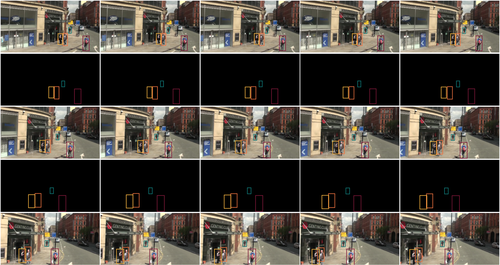
\includegraphics[width=1.0\textwidth]{figures/MOHART/mot_example2.png}
	\caption{Camera blackout experiment on a street scene from the MOTChallenge dataset with strong ego-motion. The reader is encouraged to compare top left and bottom right frame to make the amount of ego-motion apparent.}
	\label{fig:blackout2}
\end{figure}


In \Cref{sec:experiment_real}, we conducted a set of camera blackout experiments to test \textsc{mohart}'s capability of dealing with faulty sensor inputs. While traditional pipeline methods require careful consideration of different types of corner cases to properly handle erroneous sensor inputs, \textsc{mohart} is able to capture these automatically, especially when confronted with similar issues in the training scenarios. To simulate this, we replace subsequences of the images with black frames. \Cref{fig:blackout1} and \Cref{fig:blackout2} show two such examples from the test data together with the model's prediction. \textsc{mohart} learns not to update its internal model when confronted with black frames and instead uses the LSTM to propagate the bounding boxes. When proper sensor input is available again, the model uses this to make a rapid adjustment to its predicted location and `snap' back onto the object. This works remarkably well in both the presence of occlusion (\Cref{fig:blackout1}) and ego-motion (\Cref{fig:blackout2}). \Cref{tab:results_motc,tab:results_detrac,tab:results_stanford} show that the benefit of relational reasoning is particularly high in these scenarios specifically. These experiments can also be seen as a proof of concept of \textsc{mohart}'s capabalities of predicting future trajectories---and how this profits from relational reasoning.